% !TEX root =  master.tex
\chapter{Time Series Forecasting}
\label{ch:forecasting}

Time series forecasting is a statistical technique used to predict future values based
on previously observed values. This method is particularly valuable in  fields, where
understanding and anticipating trends and patterns over time is crucial, such as
finance \parencite{andersen2005volatility}, medicine \parencite{topol2019high},
environmental science \parencite{mudelsee2019trend}, and biology \parencite{stoffer2012special}.

At its core, time series forecasting involves analyzing data points collected or
recorded at specific time intervals. These data points can represent anything from
daily stock prices and monthly sales figures to hourly weather readings and \ac{IOT}
sensor data. The primary objective is to use this historical data to make informed
predictions about future events, trends, or behaviors \parencite[ch. 1]{zhang2001investigation}.

One of the key characteristics of time series data is that the observations are
sequentially dependent. This temporal ordering introduces a unique challenge and
opportunity: the potential to identify patterns such as seasonality, trends, and
cycles \parencite{assfalg2009periodic}. For example, retail sales data often
exhibit seasonal patterns, with higher sales during holidays, while economic
indicators might show long-term trends reflecting economic growth or decline.

This chapter aims to give a detailed overview about important terminology and
time series forecasting models.

\section{Terminology}
To understand time series forecasting, we first need to define some terminology.
A time series is a set of observations recorded over time \parencite{haben2023time},
as shown in Figure \ref{tab:time_series_example}.


\begin{table}[h]
    \centering
    \begin{tabular}{|c|c|}
        \hline
        \textbf{Timestamp} & \textbf{Feature\_1} \\
        \hline
        2000-04-01         & 100                 \\
        \hline
        2000-04-02         & 150                 \\
        \hline
        2000-04-03         & 170                 \\
        \hline
    \end{tabular}
    \caption{A simple example for a time series.}
    \label{tab:time_series_example}
\end{table}

There are two unique features in time series analysis: time-step features and lag
features \parencite{haben2023time}. Time-step features indicate the interval between
two timestamps, while lag features represent the difference in a feature metric
compared to the previous timestamp (Table \ref{tab:time_series_extended}).


\begin{table}[h]
    \centering
    \begin{tabular}{|c|c|c|c|}
        \hline
        \textbf{Timestamp} & \textbf{Feature\_1} & \textbf{Time-step} & \textbf{Lag} \\
        \hline
        2000-04-01         & 100                 & 0                  & NaN          \\
        \hline
        2000-04-02         & 150                 & 1                  & 100          \\
        \hline
        2000-04-03         & 170                 & 2                  & 150          \\
        \hline
    \end{tabular}
    \caption{A simple time series extended with the time-step and lag feature.}
    \label{tab:time_series_extended}
\end{table}

Time step features allow for modeling time dependence. For example, if the time-step
feature counts the days within the month, this can help identifying seasonal
dependencies of \textit{Feature\_1} within the month (Table \ref{tab:time_series_extended}).
On the other hand, lag features help identify serial dependence, meaning the correlation of
current feature values with past feature values. Therefore, serial dependence can test the
hypothesis whether past feature values influence current feature values.

\textcite{box2015time} defined the term autocorrelation as a measure of correlation
between the values of a time series at different time lags. A positive autocorrelation
coefficient at a certain lag indicates that high values tend to follow high values and
low values tend to follow low values, while a negative coefficient suggests that high
values follow low values and vice versa \parencite[ch. 2]{box2015time}.

\subsection{Trend}

Another commonly used term in time series forecasting is the ``trend''. A
trend describes a long-term change in the mean of the time series \parencite[ch. 5]{haben2023time},
as shown in Figure \ref{fig:ts_trend}.

\begin{figure}[h]
    \centering
    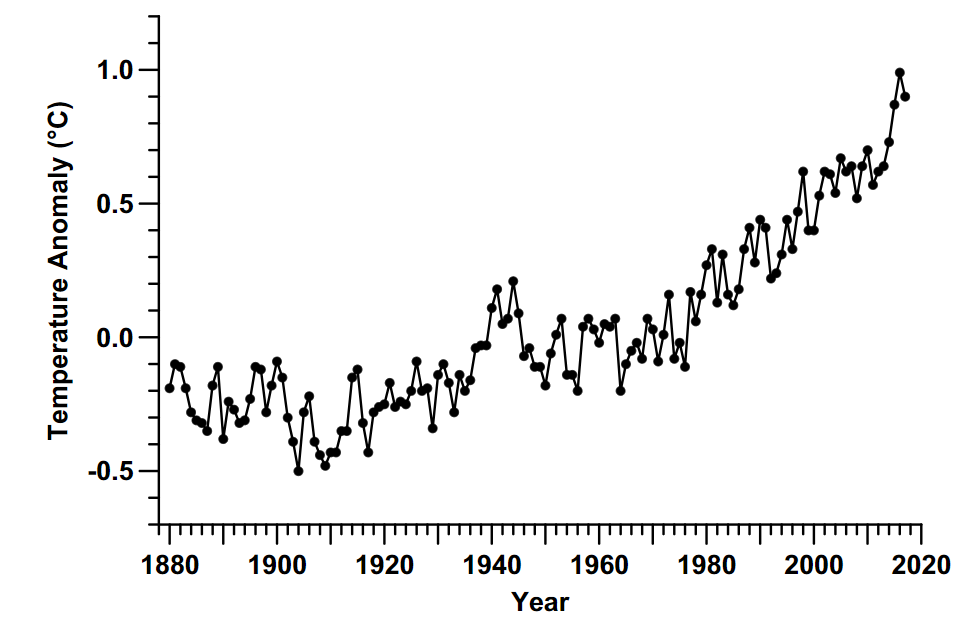
\includegraphics[width=0.75\linewidth]{img/Time Series Trend.png}
    \caption{The time series of the temperature anomaly shows a clear upwards trend
        \parencite[p. 311]{mudelsee2019trend}.}
    \label{fig:ts_trend}
\end{figure}

The trend is the slowest moving part of a time series, but it is essential
to understanding movement patterns that influence the time series. A trend can
be calculated in different ways. One common approach is the \ac{SMA}, which
calculates the mean of values within a sliding window \parencite{klinker2011exponential}.
The larger the width of the sliding window, the slower the moving average adapts
to (temporal) changes within the time series. Trends can be linear or quadratic
for instance. A more sophisticated moving average is the \ac{EMA} which places
greater significance on the most recent data points \parencite{hansun2013new}.
Unlike \ac{SMA}, which assigns equal weight to all observations in the period,
\ac{EMA} applies a weighting factor that decreases exponentially
\parencite{klinker2011exponential}. This makes \ac{EMA} more responsive to
recent price changes, which is particularly useful in financial markets for
analyzing trends and making trading decisions \parencite{dzikevivcius2010ema}.

Besides computing the trend through a moving average, we can also try to identify
it using a machine learning model, such as a linear regression. Using this trend, we
can then forecast future feature values by extending the learned function
representing the underlying trend within the data over future timestamps.

\subsection{Seasonality}
\label{subsec:seasonality}

A recurring, periodic trend is often referred to as seasonality. A seasonality
is said to occur when the mean of the series changes repeatedly in the same
point in time within a given time range, e.g., year or month \parencite{haben2023time},
as shown in Figure \ref{fig:ts_seasonality}.
Seasonality can be caused by natural cycles or societal behaviors
related to dates or times. Examples of seasonality include temperatures peaking
in summer and toy sales peaking around Christmas  \parencite{haben2023time}.

\begin{figure}[h]
    \centering
    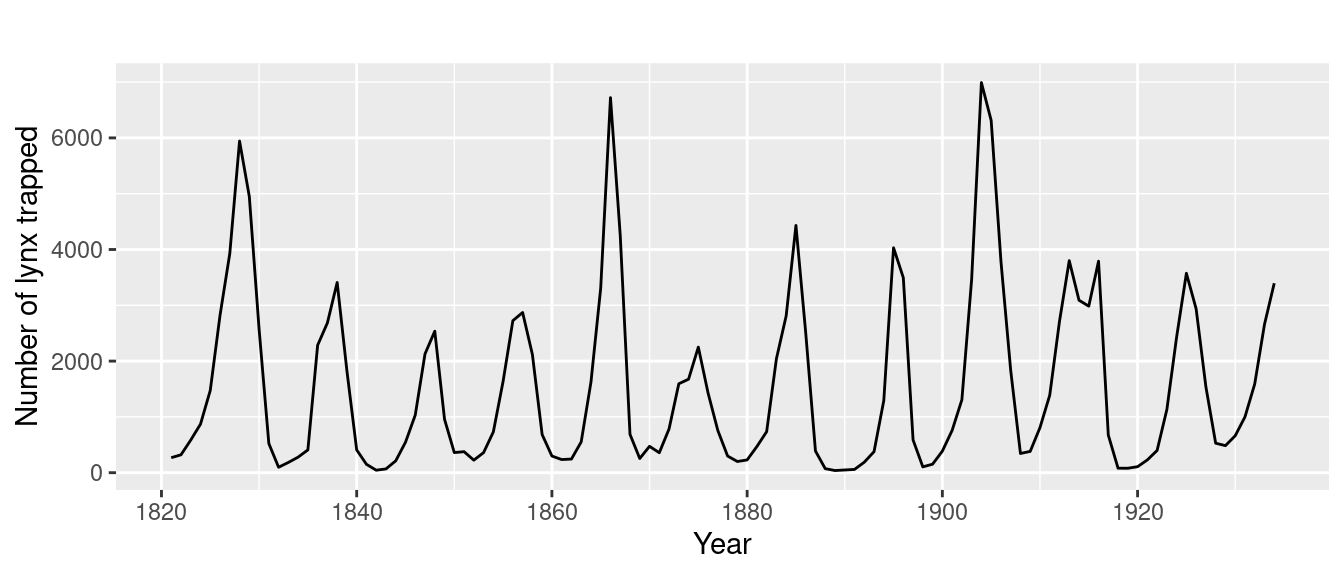
\includegraphics[width=0.75\linewidth]{img/Seasonality Time Series.png}
    \caption{A time series showing a clear example of seasonality \parencite{hyndman2011cyclic}.}
    \label{fig:ts_seasonality}
\end{figure}

To identify seasonality, seasonal plots and indicators can be used. A seasonal plot
shows segments of a time series against a consistent period,
representing the specific ``season'' you want to analyze. For instance, the values of a
feature can be plotted with the weekday on the x-axis if a weekly seasonality is
expected. Seasonal indicators can help a model distinguish means within a seasonal
period. For instance, if you expect weekly seasonality, the seasonal indicators
could be the weekdays in a one-hot-encoded format, as shown in Table \ref{tab:time_series_simple}.

\begin{table}[h]
    \centering
    \begin{tabular}{|c|c|c|c|c|c|c|}
        \hline
        \textbf{Timestamp} & \textbf{Feature\_1} & \textbf{Monday} & \textbf{Tuesday} & \textbf{Wednesday} & \textbf{Thursday} & \textbf{Friday} \\
        \hline
        2000-04-01         & 100                 & 1               & 0                & 0                  & 0                 & 0               \\
        \hline
        2000-04-02         & 150                 & 0               & 1                & 0                  & 0                 & 0               \\
        \hline
        2000-04-03         & 170                 & 0               & 0                & 1                  & 0                 & 0               \\
        \hline
        2000-04-04         & 180                 & 0               & 0                & 0                  & 1                 & 0               \\
        \hline
        2000-04-05         & 90                  & 0               & 0                & 0                  & 0                 & 1               \\
        \hline
    \end{tabular}
    \caption{A simple time series with seasonal indicators for the weekdays.}
    \label{tab:time_series_simple}
\end{table}

Note, that we can also model seasonality using sine and cosine curves to capture
multiple seasonalities within a time series. The technique which leverages these
curves to transform a time series into its constituent frequencies is called
Fourier Transformation \parencite[ch. 1]{bloomfield2004fourier}. By decomposing
a time series into a sum of sine and cosine functions, it enables the identification
and characterization of various cyclical patterns within the data. \ac{FFT} is
an efficient algorithm that computes the Fourier Transformation, making
it feasible to apply this method to large datasets in real-time applications
\parencite[ch. 5]{bloomfield2004fourier}. This approach allows for a more nuanced
understanding and forecasting of time series data by isolating and analyzing
recurring patterns across different temporal scales.

\subsubsection*{Cyclic Time Series}
Another notable mention is cyclic time series, a type of data sequence characterized
by periodic fluctuations that occur over irregular intervals, often spanning several
years. Unlike seasonal variations, which follow a regular, predictable pattern within
a year, cyclic patterns are influenced by broader economic, social, or environmental
factors and do not have a fixed period \parencite[p.4102]{gharehbaghi2017deep}.
Possible reasons for those cycles are long-term influences such as business cycles,
economic expansions, and recessions.

\section{Forecasting}
\label{sec:Forecasting}
Time series forecasting is a statistical method used to predict future values based
on previously observed data points \parencite[ch. 5]{box2015time}. While there are
methods such as \ac{ARIMA} or exponential smoothing \parencite[ch. 5]{box2015time},
machine learning algorithms can also be employed to analyze the dependencies and
relationships between different time points. This allows us to learn from historical
data in order to predict future values. Generally, these machine learning algorithms
optimize their model parameters to minimize
forecasting errors \parencite[ch. 5]{box2015time}. Which parameters they optimize is
dependent on the underlying model. Popular models will be covered in Chapter
\ref{sec:forecasting_models}.

Typical examples for those forecasting erros are: the \ac{MAE}, which calculates
the average absolute difference between the predicted values and the actual values;
the \ac{MSE}, which computes the average of the squared differences between the
predicted and actual values (squaring the errors penalizes larger errors more
significantly, making MSE sensitive to outliers); the \ac{RMSE} which is the
square root of the \ac{MSE}, providing an error measure in the same units as
the original data and the \ac{MAPE} which expresses the error as a percentage
of the actual values, which can be useful for comparing forecast accuracy across
different datasets or scales.

For regression models, a common metric is the R-squared (R2) Score, which
indicates how well the model's predictions approximate the variance in the data compared
to a simple mean prediction. The R-squared Score ranges from 0 to 1, where 1
indicates a perfect fit. Additionally, the R-squared Score can be adjusted to
account for the number of predictors in the model, providing a more realistic
evaluation of model fit. This adjusted metric is then referred to as the adjusted
R-squared Score.

\section{Feature Engineering}
Feature engineering is crucial in time series forecasting, involving techniques
such as partial autocorrelation and autocorrelation analysis to identify relevant
lags. Autocorrelation measures how current values in the series relate to past values,
while partial autocorrelation isolates the relationship of specific lags, which helps
in the selection of relevant features for the model \parencite{box2015time}.

Further, one can also create new features such as lagged variables, which are created
by shifting the original timeseries data by one or more periods. The lags can be created
heuristically e.g. 1, 2 and 12 months. Consequently, \ac{PACF} can be used to identify
significant lags that should be included as features \parencite[ch. 6]{hyndman2018forecasting}.
These lagged variables can be combined with rolling windows which calculate statistics
(e.g. mean, standard deviation, sum, etc.) over a specific timeframe. After creating
lagged variables, the rolling windows can be used to calculate rolling statistics on
the features and capture more complex patterns \parencite[ch. 6]{hyndman2018forecasting}.

Additionally, it may be useful to include binary or numerical features representing
the occurrence of significant external events, e.g., holidays or economic shifts
\parencite[ch. 3]{hyndman2018forecasting}. Additionally, integrating real-time data as
features relevant to the modeling domain can significantly enhance the model's predictive
accuracy and responsiveness to current trends.

\section{Forecasting Models}
\label{sec:forecasting_models}
Regarding time series forecasting models, one can distinguish between global and local
models which differ fundamentally in their scope and application \parencite{montero2021principles}.
Local models concentrate on individual time series, developing distinct models
tailored to each specific dataset. This
approach allows for highly customized forecasts tailored to the specific patterns and
characteristics of each series, often yielding high accuracy for single series predictions.
However, local models can be resource-intensive, demanding substantial computational power and
specialized expertise to develop and maintain multiple individualized models. In contrast,
global models aggregate
multiple time series into a single model, leveraging shared patterns and trends across datasets.
This approach can be more efficient, as it reduces the need for multiple models and can
improve scalability. Global models are particularly effective when individual series
exhibit similar behaviors, allowing the model to learn from a broader context. However,
they may not capture the unique nuances of each series as effectively as local models.
Ultimately, the choice between local and global time series forecasting depends on the
specific requirements of the application, including the number of series to forecast,
computational resources, and the need for individualized predictions
\parencite{montero2021principles}. Examples of local and global models can be found in
Table \ref{tab:timeseries_models}.

\begin{table}[h]
    \centering
    \begin{tabular}{ll}
        \toprule
        \textbf{Model type}                                          & \textbf{Can be used for} \\
        \midrule
        Linear Regression                                            & Local                    \\
        \midrule
        ARIMA                                                        & Local                    \\
        \midrule
        ETS                                                          & Local                    \\
        \midrule
        Tree-based (Decision Tree, Random Forest, Gradient Boosting) & Local/Global             \\
        \midrule
        RNN                                                          & Local/Global             \\
        \midrule
        LSTM                                                         & Local/Global             \\
        \midrule
        Transformer-based                                            & Global                   \\

        \bottomrule
    \end{tabular}
    \caption{Timeseries Forecasting Models}
    \label{tab:timeseries_models}
\end{table}

There are various algorithms with which a time series forecasting problem can be
solved \parencite{salinas2020deepar}. Regression algorithms, such as linear and
polynomial regression, are foundational techniques that model the relationship
between independent variables and the target variable, providing interpretable
and straightforward forecasts. Tree-based methods, including decision trees,
random forests, and gradient boosting machines, are powerful for handling complex,
non-linear relationships and interactions among features, often delivering robust
performance with less need for extensive data preprocessing. \ac{RNNs} excel in
time series forecasting due to their ability to maintain memory of previous inputs,
making them suitable for capturing temporal dependencies. \ac{LSTM} networks, an
advanced form of \ac{RNNs}, further enhance forecasting capabilities by addressing
the vanishing gradient problem, enabling the model to learn and retain long-term
dependencies more effectively. Each of these algorithms can be tailored to specific
forecasting challenges, with selection depending on factors such as data characteristics,
desired interpretability, and computational resources.

Additionally, deep learning frameworks have significantly advanced time series
forecasting by offering sophisticated methods for modeling complex patterns and
dependencies. Frameworks like DeepAR \parencite{salinas2020deepar} and DeepVAR
\parencite{cheng2020deepvar} are notable examples. DeepAR utilizes auto-regressive
\ac{RNNs} to provide probabilistic forecasts, excelling in
scenarios with large datasets by learning from the historical data of all time
series in the dataset, thereby capturing shared patterns and improving forecast
accuracy. DeepVAR extends this approach by incorporating multivariate time series
data, allowing the model to understand and leverage the interdependencies between
multiple series for more nuanced predictions. Recently, zero-shot time series
forecasting with \ac{LLM}s such as Chronos \parencite{ansari2024chronos} has
emerged as a cutting-edge approach. Chronos leverages pre-trained \ac{LLM}s to
forecast time series without the need for task-specific training, utilizing the
model's ability to generalize from vast amounts of data. This approach can
significantly reduce the time and computational resources required for model
development, making it an attractive option for rapid deployment in diverse
forecasting scenarios.

\subsection*{Hybrid Models}
Hybrid models are sophisticated systems that integrate at least two distinct modeling approaches.
By combining the strengths of each model, hybrid models effectively mitigate their individual
weaknesses. This technique involves training the first model on the original time series data
and then training the second model on the residuals (errors) of the first model. The final
prediction is obtained by adding the outputs of both models. A crucial aspect is that each
model focuses on different features. For instance, if the first model is designed to predict
the trend, the second model does not need to include trend-related features. Some hybrid
models consist of several components; for example, a model could include separate components
for predicting the trend, yearly seasonality, weekly seasonality, and cycles
\parencite{zunic2020application}. Ensemble models that combine the results from
multiple underlying models in this manner are often referred to as additive models.

A popular example of such an additive model is Facebook Prophet by \textcite{prophetpaper}.
The ensemble comprises multiple models, each specializing in predicting different aspects of the data.
The first model predicts the trend, which could be piecewise linear (allowing for multiple
changepoints, in which the growth rate can change) or logistic. The second model accounts
for the seasonality component (yearly, weekly or daily) using the Fourier series (see
chapter \ref{subsec:seasonality}). Thirdly, one of the models accounts for holiday effects,
as holidays can cause significant deviations from the usual patterns. The user can input a
list of holidays and the model will include their effects. Moreover, Prophet can include
additional regressor effects if the user provides external factors that are believed to
affect the time series. This results in the equation:

$$y(t) = g(t)+s(t)+h(t)+\epsilon(t)$$

where $y(t)$ is the observed value at time $t$, $g(t)$ is the trend component, $s(t)$ is
the seasonality component, $h(t)$ is the holiday effect and $\epsilon(t)$ is the error term,
capturing noise and other unexplained variability \parencite{prophetpaper}.

